\documentclass{beamer}
\usetheme{CambridgeUS}
\usecolortheme{beaver}

\usepackage[utf8]{inputenc}
\usepackage[spanish]{babel}
\usepackage{amsmath}
\usepackage{amssymb}
\usepackage{graphicx}
\usepackage{booktabs}
\usepackage{array}

% La figura del pipeline vive en la raiz del proyecto
\graphicspath{{./}{../../}{../paper/}}

\title{Framework de Explicabilidad Agnóstica al Modelo}
\subtitle{Para la Predicción de Series Temporales Financieras\\
\small Avance de tesis, Capítulos 1 a 3}
\author{Rushell Vanessa Zavalaga Orozco}
\institute{Escuela de Ciencia de la Computación\\
Universidad Nacional de San Agustín de Arequipa}
\date{}

\begin{document}

% =============================================================================
% PRESENTACION
% =============================================================================
\begin{frame}
    \titlepage
\end{frame}

\begin{frame}{Contenido}
    \begin{enumerate}
        \item \textbf{Capítulo 1. Introducción.} Contexto, motivación,
        planteamiento del problema, justificación y objetivos.
        \vspace{0.3cm}
        \item \textbf{Capítulo 2. Marco Teórico.} De la serie temporal
        financiera a la evaluación de una explicación.
        \vspace{0.3cm}
        \item \textbf{Capítulo 3. Estado del Arte.} Trabajos de los
        últimos cinco años (2021 a 2026).
    \end{enumerate}
\end{frame}

% =============================================================================
% CAPITULO 1. INTRODUCCION
% =============================================================================
\section[Capítulo 1]{Capítulo 1. Introducción}

\begin{frame}{La idea de la tesis en un ejemplo}
    \small
    \begin{enumerate}
        \item Un \textbf{modelo} recibe los datos de los \textbf{últimos
        20 días} del índice S\&P 500 y predice el valor del \textbf{día
        siguiente}. Cada día se describe con 15 datos (precios, volumen e
        indicadores calculados sobre ellos).
        \vspace{0.15cm}
        \item El modelo dice \emph{``mañana el índice sube''}, pero no dice
        \textbf{por qué}. Es una \textbf{caja negra}.
        \vspace{0.15cm}
        \item Quien decide con esa predicción necesita saber si se apoyó
        en algo razonable.
    \end{enumerate}
    \begin{block}{Lo que hace esta tesis}
        Construye un método que, para cada predicción, indica
        \textbf{qué dato influyó y de qué día}. Por ejemplo, ``pesó mucho
        el volumen de hace 3 días y casi nada el cierre de hace 10
        días''.
    \end{block}
    \begin{center}
        \footnotesize
        El resultado es una tabla de importancias, una fila por día y
        una columna por dato.
    \end{center}
\end{frame}

\begin{frame}{Vocabulario financiero y datos que se usan}
    \footnotesize
    \renewcommand{\arraystretch}{1.15}
    \begin{tabular}{@{}>{\raggedright\arraybackslash}p{3.0cm}>{\raggedright\arraybackslash}p{7.4cm}@{}}
    \toprule
    \textbf{Término} & \textbf{Significado} \\
    \midrule
    S\&P 500 & Índice con el valor de las 500 mayores empresas de EE.UU. Se
    usan sus datos diarios de 2010 a 2024 (3\,754 días). \\
    Portafolio & Conjunto de inversiones (acciones, bonos) de una persona o
    institución. \\
    Precio de cierre & Valor del índice al terminar el día. Apertura, máximo y
    mínimo son los otros precios del día, y el volumen es cuánto se negoció. \\
    Indicador técnico & Cálculo sobre precios pasados, por ejemplo la media de
    los últimos 5 días (SMA-5) o el RSI, que mide si el precio subió muy
    rápido. \\
    Retorno logarítmico & Variación relativa del precio entre dos días,
    $\ln(P_{t+1}/P_t)$. \\
    Mercado alcista y bajista & Tramos donde el precio sube (2023 y 2024) o
    cae (2022) de forma sostenida. \\
    Ventana de entrada & Los últimos $T=20$ días con $V=15$ datos cada uno,
    una tabla de $20\times15$. \\
    \bottomrule
    \end{tabular}
\end{frame}

\begin{frame}{Contexto}
    \begin{itemize}
        \item Un \textbf{portafolio} es el conjunto de inversiones de una
        persona o institución. Se predice, por ejemplo, el precio de cierre
        de un índice para decidir cuándo comprar, mantener o vender
        (Arsenault et al., 2025).
        \vspace{0.2cm}
        \item \textbf{Riesgo de mercado.} Perder dinero porque el precio se
        movió en contra, aunque el modelo se entendiera bien.
        \vspace{0.2cm}
        \item \textbf{Riesgo de modelo.} Perder dinero porque se decidió con
        un modelo incorrecto o mal usado. Lo define el \textbf{SR~11-7}, la
        guía de la Reserva Federal de EE.UU. (2011) que exige a los bancos
        gestionar sus modelos.
        \vspace{0.2cm}
        \item La opacidad lo agrava (Cohen et al., 2023), porque no se
        sabe si el modelo aprendió una relación real o una coincidencia
        espuria.
        \vspace{0.25cm}
        \item \textbf{Esta tesis se ubica en el riesgo de modelo}, no en
        el riesgo de mercado.
    \end{itemize}
\end{frame}

\begin{frame}{Motivación}
    \begin{itemize}
        \item El aprendizaje profundo reduce el error frente a los
        métodos clásicos (Bhandari et al., 2022; Abdul Quadir et al., 2023).
        \vspace{0.2cm}
        \item Pero \textbf{no explica} sus resultados, y la regulación
        ya lo exige.
        \begin{itemize}
            \item SR~11-7 (guía de la Reserva Federal). Entender los
            límites del modelo antes de usarlo.
            \item Reglamento de IA de la UE (2024). Transparencia en
            usos como el crédito.
            \item Sovrano et al.\ (2026). Los métodos actuales aún no
            cumplen de forma sistemática.
        \end{itemize}
        \vspace{0.2cm}
        \item Un modelo que no se explica no se puede auditar.
        \vspace{0.35cm}
        \item \textbf{Pregunta central.} ¿Qué variable fue relevante y
        \emph{cuándo} lo fue?
    \end{itemize}
\end{frame}

\begin{frame}{Planteamiento del Problema}
    \begin{block}{El problema}
        Los modelos que predicen series financieras no explican
        \textbf{qué dato de qué día} influyó en cada predicción.
    \end{block}
    \begin{block}{Qué se necesita}
        \begin{enumerate}
            \item Que funcione con \textbf{cualquier modelo}, sin acceder
            a su interior.
            \item Que \textbf{respete el orden temporal} de los datos.
            \item Un \textbf{costo fijo por predicción}, sin optimizar
            nada cada vez.
        \end{enumerate}
    \end{block}
    \begin{alertblock}{Por qué sigue sin resolverse}
        \begin{itemize}
            \item Los métodos que sirven con cualquier modelo tratan cada
            día como un dato suelto y \textbf{rompen el orden temporal}.
            \item Los que sí respetan el orden \textbf{necesitan el
            gradiente} del modelo, así que no sirven para Random Forest.
            \item Ninguno se validó en series financieras.
        \end{itemize}
    \end{alertblock}
    \begin{center}
        \footnotesize Los métodos concretos se detallan en el Capítulo 3.
    \end{center}
\end{frame}

\begin{frame}{Justificación}
    \begin{itemize}
        \item \textbf{Costo fijo.} Perturbar una celda no depende de
        otra, así que todas caben en \textbf{un solo batch}. Los métodos
        con gradiente, en cambio, son secuenciales.
        \vspace{0.2cm}
        \item \textbf{Cierra la brecha.} Una celda a la vez, orden
        temporal intacto y sin gradientes.
        \vspace{0.2cm}
        \item \textbf{Caso concreto.} Random Forest es competitivo en
        datos tabulares (Grinsztajn et al., 2022) y esta línea lo
        excluye.
        \vspace{0.2cm}
        \item \textbf{Responsabilidad.} Se reportan también los
        resultados desfavorables, y sin gradientes baja la barrera de
        cómputo para auditar.
    \end{itemize}
\end{frame}

\begin{frame}{Objetivo General}
    \begin{center}
        \vspace{0.4cm}
        \normalsize
        Desarrollar un framework de explicabilidad temporal
        \textbf{agnóstico al modelo} para la predicción de series
        temporales financieras, que atribuya importancia por
        \textbf{variable y paso de tiempo}
        ($\hat{\alpha} \in \mathbb{R}^{T \times V}$) sin depender de la
        estructura interna del modelo ni requerir sus gradientes, con un
        \textbf{costo fijo por instancia} evaluable en una sola pasada.
    \end{center}
\end{frame}

\begin{frame}{Pipeline del Framework}
    \begin{center}
        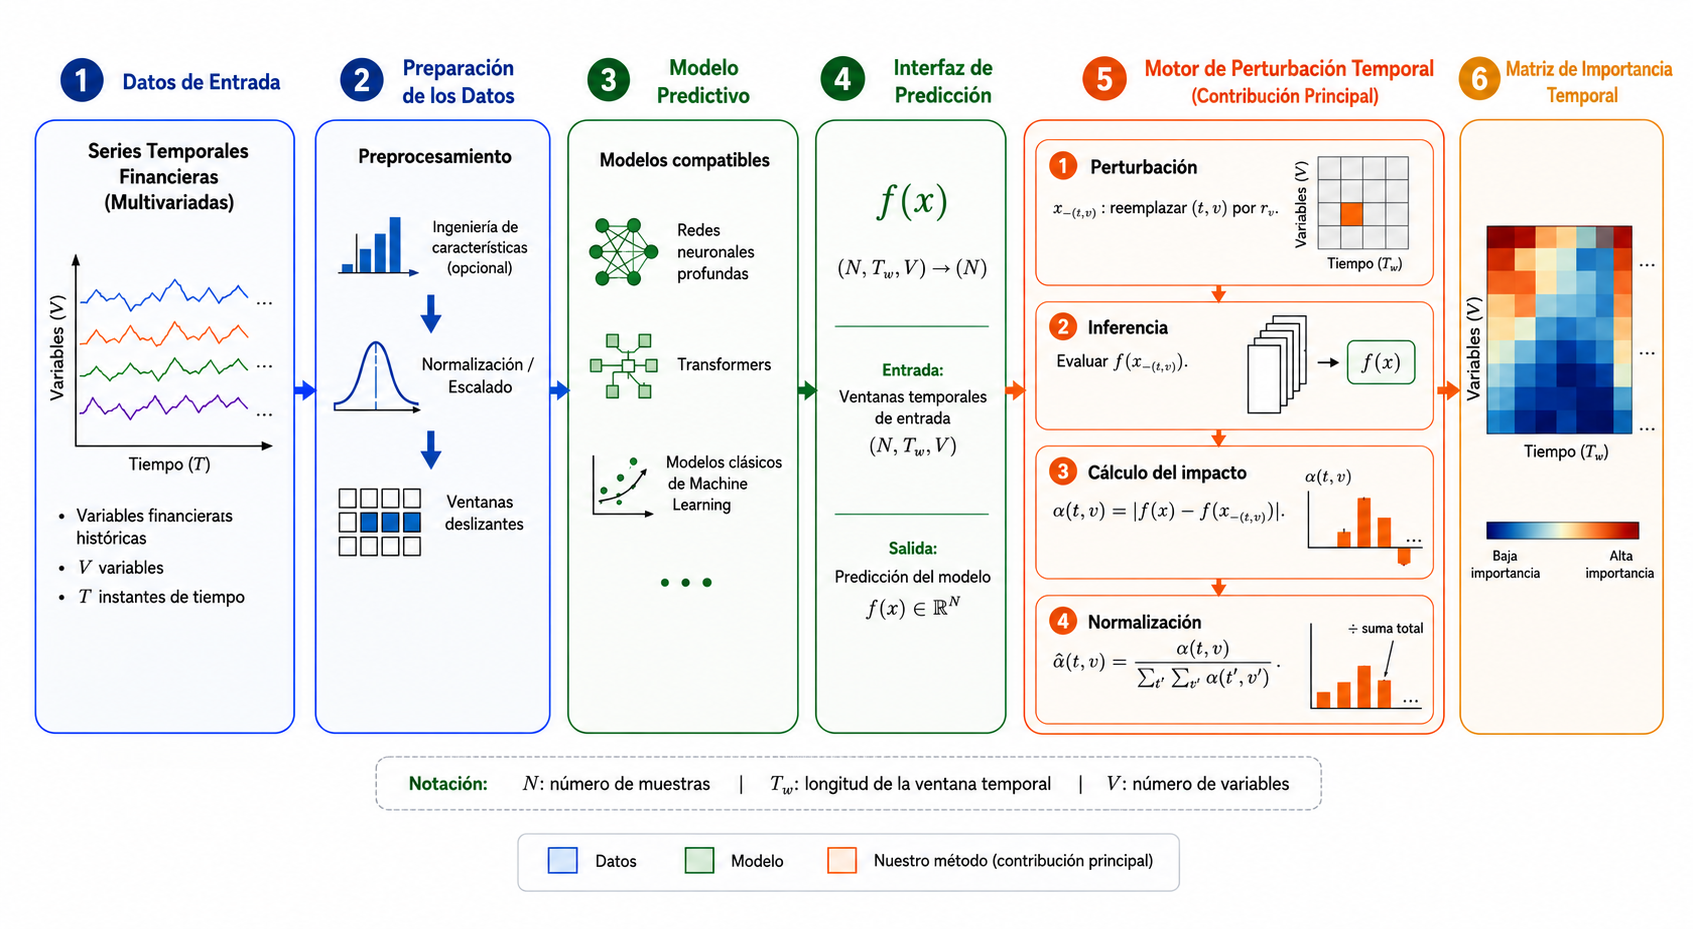
\includegraphics[width=\linewidth]{PIPELINE.png}
    \end{center}
    \begin{center}
        \scriptsize
        (1) Datos $\to$ (2) Preparación $\to$ (3) Modelo $\to$
        (4) Interfaz de predicción $\to$ (5) Motor de perturbación
        $\to$ (6) Matriz $\hat{\alpha}$
    \end{center}
\end{frame}

\begin{frame}{Objetivos Específicos}
    \begin{enumerate}
        \item \textbf{Diseñar} una interfaz uniforme de predicción, con
        un adaptador de dos niveles.
        \vspace{0.15cm}
        \item \textbf{Formular} un motor de perturbaciones por celda
        $(t,v)$, con orden temporal intacto y un único batch.
        \vspace{0.15cm}
        \item \textbf{Entrenar} LSTM, Transformer y Random Forest sobre
        el S\&P 500.
        \vspace{0.15cm}
        \item \textbf{Verificar} que las explicaciones reflejan el
        comportamiento de cada modelo.
        \vspace{0.15cm}
        \item \textbf{Evaluar} frente al estado del arte agnóstico, en
        precisión, consistencia y velocidad.
    \end{enumerate}
\end{frame}

% =============================================================================
% CAPITULO 2. MARCO TEORICO
% =============================================================================
\section[Capítulo 2]{Capítulo 2. Marco Teórico}

\begin{frame}{Serie temporal financiera y ventana de entrada}
    \small
    \begin{itemize}
        \item Una serie temporal multivariada reúne varias variables
        medidas en cada instante (Tsay, 2010). El modelo no recibe la
        serie completa, recibe una \textbf{ventana} de $T$ pasos:
    \end{itemize}
    \[
        x = \begin{pmatrix}
        x_{\tau-T+1,1} & \cdots & x_{\tau-T+1,V}\\
        \vdots & \ddots & \vdots\\
        x_{\tau,1} & \cdots & x_{\tau,V}
        \end{pmatrix} \in \mathbb{R}^{T\times V}
    \]
    \begin{itemize}
        \small
        \item Un modelo predictivo es $f\colon\mathbb{R}^{T\times V}
        \to\mathbb{R}$, con $\hat{y}=f(x)$ la predicción del instante
        siguiente (Lim y Zohren, 2021).
        \item Cada celda $(t,v)$ es una variable en un paso de tiempo, y
        es la \textbf{unidad sobre la que se atribuye importancia}.
    \end{itemize}
\end{frame}

\begin{frame}{Modelos de distinta naturaleza computacional}
    \small
    \begin{center}
    \renewcommand{\arraystretch}{1.25}
    \begin{tabular}{@{}p{2.7cm}p{4.6cm}c@{}}
    \toprule
    \textbf{Modelo} & \textbf{Cómo procesa la ventana} &
    \textbf{Diferenciable} \\
    \midrule
    LSTM & Recurrente, paso a paso (Hochreiter y Schmidhuber, 1997) & Sí \\
    Transformer & Autoatención entre todos los pasos (Vaswani et al., 2017;
    Wen et al., 2023) & Sí \\
    Random Forest & Promedio de árboles, sin noción de secuencia, recibe
    $T\cdot V$ atributos (Breiman, 2001) & No \\
    \bottomrule
    \end{tabular}
    \end{center}
    \vspace{0.2cm}
    \begin{itemize}
        \footnotesize
        \item La salida de un bosque queda dentro del rango de los
        valores objetivo vistos al entrenar, por eso no puede extrapolar.
        Esa es una razón para entrenar sobre retornos y no sobre precios.
        \item Que los dos primeros sean diferenciables y el tercero no
        decide \textbf{qué métodos de atribución sirven para cada uno}.
    \end{itemize}
\end{frame}

\begin{frame}{Explicabilidad y agnosticismo}
    \footnotesize
    \begin{itemize}
        \item \textbf{Interpretabilidad.} Presentar el comportamiento del
        modelo en términos comprensibles para una persona (Doshi-Velez y
        Kim, 2017).
        \item Dos ejes (Guidotti et al., 2018). Explicaciones
        \textbf{locales} (una predicción) o \textbf{globales} (el modelo
        completo), y métodos \textbf{post-hoc} sobre modelos ya entrenados.
        Esta tesis produce explicaciones locales y post-hoc.
        \item \textbf{Método agnóstico.} Trata al modelo como caja negra
        que solo se consulta (Ribeiro et al., 2016).
        \item Pero ser agnóstico por diseño no basta. Adebayo et al.\
        (2018) mostraron que varios métodos dan explicaciones casi
        idénticas incluso con los pesos del modelo aleatorizados.
        Rudin (2019) añade que una explicación post-hoc no es
        completamente fiel. Por eso \textbf{la fidelidad se mide, no se
        supone}.
        \item Criterio adoptado. Si el método es fiel, las explicaciones
        deben \emph{cambiar} entre modelos de distinta naturaleza.
    \end{itemize}
\end{frame}


\begin{frame}{Familias de métodos de atribución}
    \footnotesize
    \begin{block}{Basados en gradientes}
        Usan la derivada de la salida respecto de la entrada (Simonyan et
        al., 2014). Integrated Gradients integra gradientes entre una
        referencia y la entrada (Sundararajan et al., 2017).
        \textbf{Requieren un modelo diferenciable}, así que no aplican a
        Random Forest.
    \end{block}
    \begin{block}{Basados en atención}
        Leen los pesos de atención como importancia. Dependen de la
        arquitectura, y Jain y Wallace (2019) muestran que esos pesos
        pueden cambiar sin alterar la predicción.
    \end{block}
    \begin{alertblock}{Basados en perturbación}
        Modifican parte de la entrada y observan cómo cambia la salida
        (Zeiler y Fergus, 2014; Ribeiro et al., 2016). Solo consultan el
        modelo, por lo que son agnósticos. Su costo son varias consultas
        por explicación. \textbf{Es la familia de la propuesta.}
    \end{alertblock}
\end{frame}

\begin{frame}{Métodos de perturbación}
    \footnotesize
    \begin{itemize}
        \item \textbf{Oclusión.} Se reemplaza la celda $(t,v)$ por una
        referencia $r_v$ y se mide el cambio en la predicción
        (Zeiler y Fergus, 2014):
    \end{itemize}
    \[
        \alpha(t,v) = \bigl|\,f(x) - f(x_{-(t,v)})\,\bigr|
    \]
    \begin{itemize}
        \item La \textbf{referencia} define qué es ausencia de
        información (media de entrenamiento, cero, valor previo). Cambiarla
        puede cambiar la atribución, por lo que su sensibilidad se mide.
        \item \textbf{Valores de Shapley} (Shapley, 1953). Contribución
        promedio de cada variable sobre todas las coaliciones. SHAP
        (Lundberg y Lee, 2017) los unifica y el cálculo exacto crece de
        forma exponencial, por eso se aproxima por muestreo (Castro et
        al., 2009).
        \item \textbf{LIME} (Ribeiro et al., 2016). Ajusta un modelo
        lineal local sobre perturbaciones de la instancia.
        \item \textbf{Limitaciones.} Suponen variables independientes, lo
        que falla en series temporales, y la entrada perturbada puede caer
        fuera de la distribución de entrenamiento (Hooker et al., 2021).
    \end{itemize}
\end{frame}

\begin{frame}{Explicabilidad temporal}
    \small
    \begin{itemize}
        \item Extiende la atribución a la dimensión del tiempo. Produce
        una matriz $\hat{\alpha}\in\mathbb{R}^{T\times V}$ que responde a
        la vez \textbf{qué variable} influyó y \textbf{cuándo}
        (Tonekaboni et al., 2020; Rojat et al., 2021).
        \vspace{0.12cm}
        \item Aplicar métodos pensados para imágenes o texto da
        resultados poco confiables. Ismail et al.\ (2020) muestran que
        mezclan el eje del tiempo con el de las variables.
        \vspace{0.12cm}
        \item Requisitos de una explicación temporal válida.
        \begin{itemize}
            \item Respetar el \textbf{orden temporal}, sin usar
            información futura para explicar un instante pasado.
            \item Distinguir la \textbf{dependencia entre pasos} del
            \textbf{efecto retrasado} (Leung et al., 2023).
        \end{itemize}
        \vspace{0.12cm}
        \item Un método que perturba cada paso de forma aislada ignora
        ambos efectos.
    \end{itemize}
\end{frame}


\begin{frame}{Evaluación de explicaciones}
    \small
    \begin{itemize}
        \item \textbf{Con verdad conocida.} En datos sintéticos se
        conoce el conjunto $A$ de celdas relevantes. AUP y AUR miden
        precisión y cobertura frente a $A$ (Crabbé y Van Der Schaar, 2021).
        \vspace{0.12cm}
        \item \textbf{Fidelidad.} La curva AOPC elimina primero las celdas
        más importantes y mide cuánto cae la predicción (Samek et al.,
        2017).
        \vspace{0.12cm}
        \item \textbf{Sin verdad conocida} (series reales).
        \begin{itemize}
            \item Correlación de Spearman entre matrices de modelos
            distintos (Spearman, 1904).
            \item Prueba de Mann-Whitney frente a una asignación
            aleatoria (Mann y Whitney, 1947).
            \item Estabilidad frente a la referencia, el orden y el
            régimen, siguiendo las pruebas de sensatez de Adebayo et al.\
            (2018).
        \end{itemize}
    \end{itemize}
\end{frame}

% =============================================================================
% CAPITULO 3. ESTADO DEL ARTE
% =============================================================================
\section[Capítulo 3]{Capítulo 3. Estado del Arte}

\begin{frame}{Estado del Arte: criterio de organización}
    \small
    \begin{itemize}
        \item \textbf{Ventana temporal.} Solo trabajos de los últimos
        cinco años, de 2021 a 2026. Los trabajos fundacionales anteriores
        se presentaron en el Marco Teórico.
        \vspace{0.15cm}
        \item \textbf{Criterio mecánico, no cronológico.} Cada trabajo se
        ubica según cómo construye la explicación.
        \begin{itemize}
            \item \textbf{Eje 1.} Perturbación agnóstica sin diseño
            temporal.
            \item \textbf{Eje 2.} Frameworks temporalmente conscientes,
            incluido el linaje de DynaMask.
            \item \textbf{Eje 3.} Explicadores aprendidos, con cuello de
            botella de información y contrafactuales.
        \end{itemize}
        \vspace{0.15cm}
        \item Una limitación se plantea solo si el trabajo reclamaba la
        propiedad que se le exige.
    \end{itemize}
\end{frame}

\begin{frame}{Eje 1. Perturbación agnóstica y supuesto de independencia}
    \small
    \begin{itemize}
        \item \textbf{Yadav y Subbian (2025).} Diagnostican por qué
        gradiente, oclusión y permutación fallan en predicción dinámica,
        donde romper la dependencia temporal corrompe la cadena de
        predicciones.
        \item \textbf{Huang et al.\ (2025), ShapeX.} Shapley sobre
        \emph{shapelets} en vez de puntos. Está diseñado para
        clasificación, donde la forma del patrón es la evidencia de la
        etiqueta. En regresión multivariada dos variables del mismo
        instante pueden tener roles causales independientes que un
        segmento diluye.
        \item \textbf{Aplicaciones financieras} (Gupta et al., 2025;
        Sathyampeth et al., 2025; Manikrao et al., 2026; Jagannathan et
        al., 2025; Kumar et al., 2024; Singh y Dhir, 2025; Muhammad et al.,
        2024). Usan SHAP o LIME directamente sobre ventanas, sin verificar
        si las atribuciones respetan el orden causal de la serie.
    \end{itemize}
\end{frame}

\begin{frame}{Eje 2a. Frameworks temporales con remoción o Shapley}
    \footnotesize
    \begin{itemize}
        \item \textbf{WinIT} (Leung et al., 2023). Remoción de
        observaciones para capturar efectos retrasados, sin gradientes.
        Evaluado solo en arquitecturas recurrentes y tareas clínicas.
        \vspace{0.1cm}
        \item \textbf{TimeSHAP} (Bento et al., 2021). Importancia por
        evento, celda y característica, pero limitado a modelos
        secuenciales.
        \vspace{0.1cm}
        \item \textbf{TsSHAP} (Raykar et al., 2023). Características
        definidas por el usuario, diseñado para predicción univariada.
        \vspace{0.1cm}
        \item \textbf{Roshinta y Szűcs (2026).} Ventanas dinámicas con
        PCA y atribuciones reconstruidas, evaluado en GRU y LSTM.
        \vspace{0.1cm}
        \item \textbf{GS-SHAP} (Kim y Park, 2026, preprint). Agrupa
        variables y segmentos, pierde resolución por variable individual.
    \end{itemize}
\end{frame}

\begin{frame}{Eje 2b. DynaMask, el trabajo más cercano}
    \footnotesize
    \begin{itemize}
        \item \textbf{DynaMask} (Crabbé y Van Der Schaar, 2021) aprende una
        máscara $m\in[0,1]^{T\times V}$ y un operador de perturbación
        $\pi$ fijo (difuminado, media móvil, valor pasado):
    \end{itemize}
    \[
        \Phi_m(x)=m\odot x+(1-m)\odot\pi(x),\qquad
        \mathcal{L}(m)=\mathcal{L}_e+\lambda_a\mathcal{L}_a+\lambda_c\mathcal{L}_c
    \]
    \begin{itemize}
        \item Su salida es una matriz $T\times V$, igual que la de esta
        tesis, pero \textbf{requiere el gradiente} del modelo, no corre en
        Random Forest y su costo crece con las iteraciones por instancia.
        \item $\pi$ supone una serie localmente suave, algo que choca con
        los regímenes de mercado.
        \item \textbf{ExtrMask} (Enguehard, 2023) aprende también la
        perturbación y \textbf{ContraLSP} (Liu et al., 2024) usa
        aprendizaje contrastivo. Mantienen la dependencia del gradiente y
        ninguno de los tres se evalúa en series financieras.
    \end{itemize}
    \begin{alertblock}{Suficiencia y necesidad (Pearl, 2009)}
        Las máscaras buscan lo \emph{suficiente} para mantener la
        predicción. La oclusión mide lo \emph{necesario}, cuánto se pierde
        al quitar una celda.
    \end{alertblock}
\end{frame}

\begin{frame}{Eje 3. Explicadores aprendidos y cuello de botella}
    \small
    \begin{itemize}
        \item \textbf{TimeX} (Queen et al., 2023). Entrena un modelo
        sustituto cuyo espacio latente conserva las relaciones del modelo
        original y aprende patrones temporales recurrentes.
        \vspace{0.1cm}
        \item \textbf{TimeX++} (Liu et al., 2024). Objetivo bajo el
        principio del cuello de botella de información que evita
        soluciones triviales y el desplazamiento de distribución.
        \vspace{0.1cm}
        \item \textbf{Zheng et al.\ (2026, preprint).} Marco unificado de
        atribución y contrafactual con una red paramétrica.
        \vspace{0.2cm}
        \item \textbf{Rasgos comunes.}
        \begin{itemize}
            \item Entrenan una red auxiliar, por lo que su costo no es el
            de consultar el modelo una vez por celda.
            \item Se evalúan en benchmarks sintéticos y de dominios ajenos
            a las finanzas.
        \end{itemize}
    \end{itemize}
\end{frame}

\begin{frame}{Síntesis y brecha de investigación}
    \tiny
    \begin{center}
    \renewcommand{\arraystretch}{1.2}
    \begin{tabular}{@{}>{\raggedright\arraybackslash}p{2.6cm}>{\raggedright\arraybackslash}p{3.6cm}>{\raggedright\arraybackslash}p{3.6cm}@{}}
    \toprule
    \textbf{Referencia} & \textbf{Mecanismo y dominio} & \textbf{Brecha} \\
    \midrule
    SHAP, LIME & Perturbación genérica, datos tabulares & Asumen independencia entre pasos \\
    WinIT (2023) & Remoción de observaciones, clínico & Solo modelos recurrentes \\
    DynaMask (2021) & Máscara por gradiente, sintético y MIMIC-III & Requiere gradientes, no corre en Random Forest \\
    ExtrMask, ContraLSP & Perturbación aprendida o contrastiva & Mantienen la dependencia del gradiente \\
    TimeSHAP (2021) & Shapley sobre eventos & Solo modelos secuenciales \\
    Roshinta, GS-SHAP & Ventanas dinámicas, agrupación & Pierden resolución por variable, un solo tipo de modelo \\
    TimeX, TimeX++ & Explicador aprendido, clasificación & Entrenan una red auxiliar, sin regresión financiera \\
    Zheng et al.\ (2026) & Atribución y contrafactual unificados & Requiere entrenar una red, preprint \\
    \midrule
    \textbf{Propuesta} & \textbf{Oclusión celda a celda, sin gradientes, S\&P 500, 3 modelos} & \textbf{Agnóstica, costo fijo, resolución por celda, validada en finanzas} \\
    \bottomrule
    \end{tabular}
    \end{center}
\end{frame}

\begin{frame}{La brecha que cubre esta tesis}
    \small
    \begin{alertblock}{Ningún trabajo previo satisface simultáneamente}
        \begin{enumerate}
            \item \textbf{Agnosticismo real} al modelo, sin gradientes y
            sin estructura secuencial obligatoria.
            \item \textbf{Resolución completa por celda} $(t,v)$, sin
            agrupar variables ni segmentos.
            \item \textbf{Verificación empírica} de que las explicaciones
            cambian entre modelos de distinta naturaleza (criterio de
            Adebayo et al., 2018).
        \end{enumerate}
    \end{alertblock}
    \vspace{0.2cm}
    \begin{block}{Hipótesis de trabajo}
        Es posible construir un método de perturbación temporalmente
        ordenado y agnóstico al modelo que produzca explicaciones
        consistentes con el comportamiento de cada arquitectura.
    \end{block}
    \begin{center}
        \footnotesize Siguiente capítulo, la propuesta.
    \end{center}
\end{frame}

% =============================================================================
% REFERENCIAS
% =============================================================================
\begin{frame}[allowframebreaks]{Referencias}
    \tiny
    \begin{thebibliography}{99}
        \bibitem{r1} Abdul Quadir, M.\ et al.\ (2023). Novel optimization
        approach for stock price forecasting using multi-layered
        sequential LSTM. \emph{Applied Soft Computing}.
        \bibitem{r2} Adebayo, J.\ et al.\ (2018). Sanity checks for saliency
        maps. \emph{NeurIPS}.
        \bibitem{r4} Arsenault, P.-D.\ et al.\ (2025). A survey of
        explainable AI (XAI) in financial time series forecasting.
        \emph{ACM Computing Surveys}.
        \bibitem{r6} Bento, J.\ et al.\ (2021). TimeSHAP. \emph{KDD}.
        \bibitem{r7} Bhandari, H.\ N.\ et al.\ (2022). Predicting stock
        market index using LSTM. \emph{Machine Learning with Applications}.
        \bibitem{r8} Breiman, L.\ (2001). Random forests. \emph{Machine
        Learning}, 45(1).
        \bibitem{r10} Castro, J., Gómez, D.\ y Tejada, J.\ (2009).
        Polynomial calculation of the Shapley value based on sampling.
        \emph{Computers \& Operations Research}, 36(5).
        \bibitem{r11} Cohen, S.\ N., Snow, D.\ y Szpruch, L.\ (2023).
        Black-box model risk in finance.
        \bibitem{r13} Crabbé, J.\ y Van Der Schaar, M.\ (2021). Explaining
        time series predictions with dynamic masks. \emph{ICML}.
        \bibitem{r14} Doshi-Velez, F.\ y Kim, B.\ (2017). Towards a rigorous
        science of interpretable machine learning. arXiv:1702.08608.
        \bibitem{r15} Enguehard, J.\ (2023). Learning perturbations to
        explain time series predictions. \emph{ICML}.
        \bibitem{r16} European Parliament and Council (2024). Regulation (EU)
        2024/1689 (AI Act).
        \bibitem{r18} Federal Reserve Board. Supervisory Guidance on Model
        Risk Management (SR 11-7).
        \bibitem{r19} Grinsztajn, L., Oyallon, E.\ y Varoquaux, G.\ (2022).
        Why do tree-based models still outperform deep learning on
        typical tabular data? \emph{NeurIPS}.
        \bibitem{r21} Guidotti, R.\ et al.\ (2018). A survey of methods for
        explaining black box models. \emph{ACM Computing Surveys}, 51(5).
        \bibitem{r22} Gupta, Y.\ et al.\ (2025). An interpretable framework
        for stock market forecasting using LSTM.
        \bibitem{r24} Hochreiter, S.\ y Schmidhuber, J.\ (1997). Long
        short-term memory. \emph{Neural Computation}, 9(8).
        \bibitem{r25} Hooker, G., Mentch, L.\ y Zhou, S.\ (2021). Unrestricted
        permutation forces extrapolation. \emph{Statistics and
        Computing}, 31.
        \bibitem{r26} Huang, B.\ et al.\ (2025). ShapeX. \emph{NeurIPS}.
        \bibitem{r27} Ismail, A.\ A.\ et al.\ (2020). Benchmarking deep
        learning interpretability in time series predictions.
        \emph{NeurIPS}.
        \bibitem{r28} Jagannathan, J.\ y Goditi, V.\ V.\ S.\ K.\ (2025).
        Integration of a hybrid model with XAI for stock price forecasting.
        \bibitem{r29} Jain, S.\ y Wallace, B.\ C.\ (2019). Attention is not
        explanation. \emph{NAACL}.
        \bibitem{r30} Kim, J.\ y Park, S.\ (2026). GroupSegment-SHAP.
        arXiv:2601.06114 (preprint).
        \bibitem{r31} Kumar, P.\ et al.\ (2024). Analysing forecasting of
        stock prices, an explainable AI approach. \emph{Procedia Computer
        Science}.
        \bibitem{r33} Leung, K.\ K.\ et al.\ (2023). Temporal dependencies in
        feature importance for time series prediction (WinIT).
        \emph{ICLR}.
        \bibitem{r34} Lim, B.\ y Zohren, S.\ (2021). Time-series forecasting
        with deep learning, a survey. \emph{Phil.\ Trans.\ R.\ Soc.\ A},
        379.
        \bibitem{r36} Liu, Z.\ et al.\ (2024). Explaining time series via
        contrastive and locally sparse perturbations (ContraLSP).
        \emph{ICLR}.
        \bibitem{r37} Liu, Z.\ et al.\ (2024). TimeX++. \emph{ICML}.
        \bibitem{r38} Lundberg, S.\ M.\ y Lee, S.-I.\ (2017). A unified
        approach to interpreting model predictions. \emph{NeurIPS}.
        \bibitem{r39} Mann, H.\ B.\ y Whitney, D.\ R.\ (1947). On a test of
        whether one of two random variables is stochastically larger than
        the other. \emph{Ann.\ Math.\ Statist.}, 18(1).
        \bibitem{r40} Manikrao, K.\ W.\ et al.\ (2026). An explainable AI for
        stock market prediction.
        \bibitem{r42} Muhammad, D.\ et al.\ (2024). An explainable deep
        learning approach for stock market trend prediction.
        \emph{Heliyon}.
        \bibitem{r43} Pearl, J.\ (2009). \emph{Causality}. 2.\ ed.,
        Cambridge University Press.
        \bibitem{r44} Queen, O.\ et al.\ (2023). Encoding time-series
        explanations through self-supervised model behavior consistency
        (TimeX). \emph{NeurIPS}.
        \bibitem{r45} Raykar, V.\ C.\ et al.\ (2023). TsSHAP. arXiv:2303.12316
        (preprint).
        \bibitem{r46} Ribeiro, M.\ T., Singh, S.\ y Guestrin, C.\ (2016).
        ``Why should I trust you?'' \emph{KDD}.
        \bibitem{r47} Rojat, T.\ et al.\ (2021). Explainable AI (XAI) on
        time series data, a survey. arXiv:2104.00950.
        \bibitem{r48} Roshinta, T.\ A.\ y Szűcs, G.\ (2026). Efficient XAI in
        multivariate time series. \emph{Neurocomputing}.
        \bibitem{r49} Rudin, C.\ (2019). Stop explaining black box machine
        learning models for high stakes decisions. \emph{Nature Machine
        Intelligence}, 1(5).
        \bibitem{r50} Samek, W.\ et al.\ (2017). Evaluating the visualization
        of what a deep neural network has learned. \emph{IEEE TNNLS},
        28(11).
        \bibitem{r51} Sathyampeth, C.\ et al.\ (2025). AI and XAI in stock
        market prediction.
        \bibitem{r53} Shapley, L.\ S.\ (1953). A value for $n$-person games.
        \emph{Contributions to the Theory of Games II}.
        \bibitem{r54} Simonyan, K., Vedaldi, A.\ y Zisserman, A.\ (2014). Deep
        inside convolutional networks. arXiv:1312.6034.
        \bibitem{r55} Singh, S.\ y Dhir, V.\ (2025). Cross-sector insights for
        robust stock market prediction.
        \bibitem{r56} Sovrano, F.\ et al.\ (2026). Assessing model-agnostic
        XAI methods against EU AI Act explainability requirements.
        \bibitem{r57} Spearman, C.\ (1904). The proof and measurement of
        association between two things. \emph{Am.\ J.\ Psychology}, 15(1).
        \bibitem{r58} Sundararajan, M., Taly, A.\ y Yan, Q.\ (2017).
        Axiomatic attribution for deep networks. \emph{ICML}.
        \bibitem{r59} Tonekaboni, S.\ et al.\ (2020). What went wrong and
        when? Instance-wise feature importance for time-series black-box
        models (FIT). \emph{NeurIPS}.
        \bibitem{r60} Tsay, R.\ S.\ (2010). \emph{Analysis of Financial Time
        Series}. 3.\ ed., Wiley.
        \bibitem{r61} Vaswani, A.\ et al.\ (2017). Attention is all you need.
        \emph{NeurIPS}.
        \bibitem{r63} Wen, Q.\ et al.\ (2023). Transformers in time series, a
        survey. \emph{IJCAI}.
        \bibitem{r64} Yadav, S.\ y Subbian, V.\ (2025). Failure modes of time
        series interpretability algorithms for critical care applications.
        \emph{AMIA Annual Symposium}.
        \bibitem{r65} Zeiler, M.\ D.\ y Fergus, R.\ (2014). Visualizing and
        understanding convolutional networks. \emph{ECCV}.
        \bibitem{r66} Zheng, X.\ et al.\ (2026). Towards a unified
        information bottleneck framework for time series explanations
        (preprint).
    \end{thebibliography}
\end{frame}

\end{document}
